\documentclass[12pt,a4paper]{article}
\usepackage[utf8]{inputenc}
\usepackage[spanish]{babel}
\usepackage{geometry}
\usepackage{amsmath,amssymb,amsfonts}
\usepackage{graphicx}
\usepackage{float}
\usepackage{booktabs}
\usepackage[hidelinks]{hyperref}
\usepackage[backend=biber, style=numeric, sorting=none]{biblatex}
\addbibresource{referencias.bib} % Tu archivo .bib
\geometry{top=2.5cm, bottom=2.5cm, left=3cm, right=3cm}

% Definiciones para la portada solicitada
\def \unidad{Escuela de Ingeniería en Electrónica \\ Centro Académico de Alajuela}
\def \programa{Ingeniería Electrónica}
\def \curso{EL5409 - Laboratorio de Control Automático}
\def \titulo{Sistema de Seguimiento Infrarrojo: ``El Girasol''}

\def \autores{
    Anthony Artavia Salazar\\
    asanthony15@estudiantec.cr\\
    2020036546\\
    
    \vspace{0.4cm}
    
    Kevin Joseph Berrocal Rodríguez\\
    kjosephbr@estudiantec.cr\\
    2020113094\\
    
    \vspace{0.4cm}
    
    José David Luna Herrera\\
    josedavidlh@estudiantec.cr\\
    2020114728\\
    
    \vspace{0.4cm}
    
    William Andrés Sánchez Ramírez\\
    william.a.sr@estudiantec.cr\\
    2018235622\\
    
    \vspace{0.4cm}
    
    Luis Pablo Vargas Muñoz\\
    pablovargas@estudiantec.cr\\
    2021490483
}

\def \fecha{Octubre 2026}
\def \lugar{Alajuela, Costa Rica}

\begin{document}

% Portada del documento
\begin{titlepage}
    \begin{center}
        \vspace*{0.8cm}
        
        % Espacio reservado para el logotipo del TEC
        
\includegraphics[width=0.7\linewidth]{Figuras/logo_tec.png}\\
        \vspace{0.5cm}
        \Large
        \unidad\\
        \vspace{0.2cm}
        \programa\\
        \vspace{0.2cm}
        \curso
        
        \vspace{0.8cm}
        \LARGE
        \textbf{\titulo}
            
        \vspace{0.8cm}
        \large
        \autores
            
        \vfill
        
        \lugar\\
        \fecha
        
    \end{center}
\end{titlepage}

\tableofcontents
\newpage

\begin{abstract}
Este informe presenta el modelado matemático, la identificación experimental y la propuesta de implementación de un sistema de seguimiento de luz de dos grados de libertad, correspondiente al proyecto ``El Girasol''. El sistema emplea un arreglo simétrico de cuatro fotoresistencias (LDR) divididas mediante un tabique para estimar el error de orientación y dos servomotores inteligentes Dynamixel AX-12A comandados mediante una placa ArbotiX-M para orientar el cabezal sensor de forma autónoma e inalámbrica. Se detallan la compensación y calibración óptica, los modelos de pequeña señal y acoplamiento entre ejes, la identificación dinámica de los actuadores como sistemas de segundo orden, la formulación en espacio de estados y la estructura de un controlador proporcional incremental con banda muerta.
\end{abstract}

\section{Introducción}
El control automático de sistemas orientables es fundamental en aplicaciones de seguimiento y robótica móvil. El proyecto ``El Girasol'' plantea el diseño de un sistema autónomo capaz de detectar y rastrear una fuente luminosa dentro de su esfera de operación utilizando un kit Dynamixel y un controlador ArbotiX-M con alimentación independiente por batería.

\section{Objetivos}
\subsection{Objetivo General}
Diseñar, modelar e implementar un sistema de control de dos grados de libertad capaz de ubicar y seguir una fuente luminosa mediante un arreglo de fotoresistencias y servomotores Dynamixel AX-12A.

\subsection{Objetivos Específicos}
\begin{itemize}
    \item Desarrollar el modelo matemático del arreglo de fotoresistencias, incluyendo compensación en oscuridad, calibración central, estimación de errores normalizados y análisis de acoplamiento entre ejes.
    \item Obtener el modelo dinámico de los servomotores como un sistema de segundo orden equivalente a partir de pruebas experimentales.
    \item Implementar el análisis de estabilidad y desempeño del sistema.
    \item Diseñar un controlador digital para el seguimiento robusto ante movimientos de la fuente luminosa.
\end{itemize}

\section{Marco Teórico}
El diseño de sistemas de seguimiento óptico y control de posición requiere la integración de principios de sensado optoelectrónico, modelado de sistemas dinámicos y control digital por retroalimentación. A continuación, se detallan los fundamentos teóricos que respaldan el desarrollo del proyecto.

\subsection{Sistemas de Percepción Óptica y Normalización de Señales}
Los sistemas orientados a la detección de fuentes luminosas suelen emplear arreglos diferenciales de sensores sensibles a la luz, tales como fotoresistencias (LDR), fototransistores o fotodiodos. En el caso de las fotoresistencias, su resistencia eléctrica varía en función de la irradiancia incidente y se acondiciona mediante redes resistivas (divisores de tensión) y conversión analógico-digital para generar lecturas $S_i(t)$. Debido a las tolerancias de fabricación, la no linealidad característica de estos elementos, la iluminación ambiental y las variaciones en la distancia o ángulo respecto a la fuente, las lecturas crudas se ven afectadas por offsets en oscuridad y diferencias de ganancia entre sensores. Para mitigar estos efectos, se aplican correcciones de offset en oscuridad, ganancias de calibración en un punto de referencia central y normalización diferencial respecto a la suma de señales, obteniendo una medida adimensional acotada que aproxima la desviación angular alrededor del punto de operación \cite{dorf2016modern, ogata2010modern}.

\subsection{Modelado Dinámico de Servomotores de Posición}
Los servomotores inteligentes, como los actuadores Dynamixel AX-12A, integran un lazo cerrado de control de posición interno a nivel de hardware. Desde la perspectiva de la teoría de control clásico, cuando se comandan a través de un controlador externo (como la placa ArbotiX-M), la relación entre la posición objetivo $u(t)$ y la posición real $\theta(t)$ puede aproximarse satisfactoriamente mediante una función de transferencia de segundo orden subamortiguada \cite{franklin2015feedback}. Este modelo captura de manera adecuada la ganancia estática, el tiempo de establecimiento y las oscilaciones o sobreimpulso característicos de la respuesta dinámica del motor y su carga mecánica asociada.

\subsection{Representación en Espacio de Estados}
Para sistemas multivariable o que requieren un análisis avanzado de estabilidad y control moderno, la representación en espacio de estados proporciona un marco matemático riguroso. Un sistema de segundo orden continuo se describe mediante un vector de estados $\mathbf{x}(t) = [\theta(t) \quad \dot{\theta}(t)]^T$, relacionando las derivadas de las variables físicas con las entradas de control y las salidas del sistema a través de las matrices de estado $\mathbf{A}$, $\mathbf{B}$, $\mathbf{C}$ y $\mathbf{D}$ \cite{ogata2010modern}.

\subsection{Control Proporcional Incremental y Banda Muerta}
En aplicaciones de seguimiento en tiempo real con fuentes móviles, un controlador proporcional (P) incremental resulta ventajoso porque calcula correcciones sobre la posición objetivo actual en lugar de requerir una referencia absoluta constante. Sin embargo, los sistemas físicos discretos sujetos a ruido eléctrico en los sensores sufren de vibraciones o desgaste mecánico por microcorrecciones continuas. Para solucionar esto, se implementa una función de \emph{banda muerta} (dead zone), la cual inhibe la acción de control cuando el error absoluto se encuentra por debajo de un umbral predefinido $\delta$, garantizando la estabilidad en el estado estacionario \cite{astrom2008feedback}.

\section{Descripción del Sistema Físico}
El sistema de seguimiento ``El Girasol'' está constituido por un arreglo mecatrónico de dos grados de libertad diseñado para operar de manera autónoma e inalámbrica mediante alimentación por batería. La arquitectura del sistema se divide en tres subsistemas principales:

\begin{itemize}
    \item \textbf{Subsistema de Percepción Óptica:} Consiste en un arreglo simétrico de cuatro fotoresistencias ($S_1$ a $S_4$) montadas sobre el cabezal sensor y separadas mediante un tabique divisor. Esta configuración permite contrastar la iluminación incidente entre cuadrantes y generar las lecturas analógico-digitales necesarias para estimar la desviación angular respecto a la fuente luminosa en los ejes horizontal (\emph{Pan}) y vertical (\emph{Tilt}).
    \item \textbf{Subsistema de Actuación (Planta Mecánica):} Está compuesto por dos servomotores inteligentes Dynamixel AX-12A acoplados ortogonalmente. El primer motor controla el giro horizontal (\emph{Pan} o azimut), mientras que el segundo motor gestiona la inclinación vertical (\emph{Tilt} o elevación del cabezal). Estos motores integran un controlador interno de posición y retroalimentación de estado.
    \item \textbf{Subsistema de Control Digital:} Emplea una tarjeta controladora ArbotiX-M, encargada de adquirir las señales de las cuatro fotoresistencias, ejecutar los algoritmos de compensación y control digital, y enviar los comandos de posición objetivo hacia los servomotores de manera síncrona.
\end{itemize}

\section{Nomenclatura y Glosario de Variables}
Para facilitar la lectura y comprensión del modelado matemático y la identificación experimental desarrollada en este informe, a continuación se definen los símbolos y variables principales utilizados:

\begin{itemize}
    \item $\theta_x, \theta_y$: Ángulo de giro horizontal (\emph{Pan}) y ángulo de inclinación vertical (\emph{Tilt}) del sistema $[\text{rad}]$ o $[\text{deg}]$.
    \item $\theta_{\mathrm{ref},x}, \theta_{\mathrm{ref},y}$: Posiciones angulares de referencia asociadas a la fuente luminosa $[\text{rad}]$ o $[\text{deg}]$.
    \item $\Delta\theta_x, \Delta\theta_y$: Desviaciones o errores angulares respecto a la fuente luminosa $[\text{rad}]$ o $[\text{deg}]$.
    \item $u_x, u_y$: Comandos o posiciones objetivo enviadas a los ejes horizontal y vertical $[\text{rad}]$ o pasos digitales.
    \item $S_i(t)$: Lectura obtenida mediante el convertidor analógico-digital (ADC) para el sensor LDR $i$-ésimo ($i = 1, 2, 3, 4$) $[\text{ADC}]$.
    \item $O_i$: Lectura promedio de compensación en oscuridad para el sensor $i$-ésimo $[\text{ADC}]$.
    \item $A_i, A_{i,c}$: Lectura promedio ambiental y lectura ambiental corregida respecto a oscuridad para el sensor $i$-ésimo $[\text{ADC}]$.
    \item $\overline{S}_{c,0}$: Promedio de las cuatro lecturas corregidas en oscuridad en la posición central $[\text{ADC}]$.
    \item $G_i$: Ganancia de calibración individual del sensor $i$-ésimo respecto al punto central [adim.].
    \item $U_i(t)$: Señal compensada (en oscuridad y calibración central) del sensor LDR $i$-ésimo $[\text{ADC}]$.
    \item $T(t)$: Señal total dada por la suma de las cuatro señales compensadas $U_1(t)+U_2(t)+U_3(t)+U_4(t)$ $[\text{ADC}]$.
    \item $D_x(t), D_y(t)$: Errores diferenciales normalizados horizontal y vertical [adim.].
    \item $D_{x,0}, D_{y,0}$: Errores diferenciales normalizados residuales en la posición central [adim.].
    \item $e_x(t), e_y(t)$: Errores normalizados compensados en el punto central para los ejes \emph{Pan} y \emph{Tilt} [adim.].
    \item $K_{s,x}, K_{s,y}$: Sensibilidades o ganancias estáticas equivalentes del subsistema de sensado $[\text{rad}^{-1}]$ o $[\text{deg}^{-1}]$.
    \item $\mathbf{J}$: Matriz Jacobiana de sensibilidad de pequeña señal del subsistema de sensado $[\text{rad}^{-1}]$.
    \item $C_{x\rightarrow y}, C_{y\rightarrow x}$: Porcentajes de acoplamiento cruzado entre los ejes \emph{Pan} y \emph{Tilt} $[\%]$.
    \item $G_x(s), G_y(s)$: Funciones de transferencia equivalentes de segundo orden para los ejes horizontal y vertical.
    \item $K_x, K_y$: Ganancias estáticas de los servomotores [adim.].
    \item $\omega_{nx}, \omega_{ny}$: Frecuencias naturales de los ejes horizontal y vertical $[\text{rad/s}]$.
    \item $\zeta_x, \zeta_y$: Coeficientes de amortiguamiento equivalentes [adim.].
    \item $\Theta_x(s), \Theta_y(s)$: Posiciones angulares reales en el dominio de Laplace $[\text{rad}]$.
    \item $U_x(s), U_y(s)$: Comandos de posición en el dominio de Laplace $[\text{rad}]$.
    \item $\theta_{x,r}, \theta_{y,r}$: Posiciones de referencia actualizadas para los motores $[\text{rad}]$.
    \item $K_{px}, K_{py}$: Ganancias proporcionales del controlador digital incremental [adim.].
    \item $\delta_x, \delta_y$: Umbrales de banda muerta para los errores ópticos [adim.].
    \item $\mathbf{x}, \dot{\mathbf{x}}$: Vector de estados del sistema y su derivada temporal.
\end{itemize}

\section{Modelado del Sistema}

\subsection{Definición de Variables y Coordenadas}
El sistema opera sobre dos ejes angulares principales:
\begin{itemize}
    \item $\theta_x$: Ángulo de giro horizontal (\emph{Pan}) en radianes o grados.
    \item $\theta_y$: Ángulo de inclinación vertical (\emph{Tilt}) en radianes o grados.
    \item $u_x, u_y$: Comandos de posición objetivo para los ejes horizontal y vertical.
\end{itemize}

\subsection{Modelado Dinámico de los Servomotores (Planta)}
Debido a que los servomotores AX-12A integran un controlador interno de posición, cada eje se modela como un sistema de segundo orden equivalente:
\begin{align}
G_x(s) &= \frac{\Theta_x(s)}{U_x(s)} = \frac{K_x\omega_{nx}^2}{s^2 + 2\zeta_x\omega_{nx}s + \omega_{nx}^2} \\
G_y(s) &= \frac{\Theta_y(s)}{U_y(s)} = \frac{K_y\omega_{ny}^2}{s^2 + 2\zeta_y\omega_{ny}s + \omega_{ny}^2}
\end{align}
En forma matricial para ambos ejes desacoplados:
\begin{equation}
\begin{bmatrix} \Theta_x(s)\\ \Theta_y(s) \end{bmatrix} = \begin{bmatrix} G_x(s)&0\\ 0&G_y(s) \end{bmatrix} \begin{bmatrix} U_x(s)\\ U_y(s) \end{bmatrix}
\end{equation}

\subsection{Modelo de Percepción (Arreglo de Fotoresistencias)}
El subsistema de sensado está conformado por cuatro fotoresistencias $S_1$, $S_2$, $S_3$ y $S_4$ separadas por un tabique divisor, cuyas lecturas ADC se agrupan en el vector $\mathbf{S}(t) = [S_1(t)\; S_2(t)\; S_3(t)\; S_4(t)]^T$. Para compensar las diferencias de respuesta en oscuridad, se calcula el promedio de las últimas $N=10$ muestras en oscuridad ($O_i$) y se corrige cada lectura mediante $S_{i,c}(t) = S_i(t) - O_i$.

Aunque se evaluó la lectura ambiental promedio $A_i$ y su valor corregido $A_{i,c} = A_i - O_i$, la sustracción directa de luz ambiental produjo valores negativos en ciertas posiciones angulares que afectaban los errores normalizados; por ello, la luz ambiental se emplea únicamente como referencia del entorno y la calibración se realiza en oscuridad y en posición central. A partir del promedio central corregido $\overline{S}_{c,0} = \frac{1}{4}\sum_{i=1}^{4} S_{i,c}(0)$, se define la ganancia individual $G_i = \overline{S}_{c,0}/S_{i,c}(0)$ y la señal compensada de cada sensor:
\begin{equation}
U_i(t) = G_i\left[S_i(t) - O_i\right]
\end{equation}

Definiendo la señal total $T(t) = U_1(t) + U_2(t) + U_3(t) + U_4(t)$ (verificada con $T(t) > 0$), los errores diferenciales normalizados para los ejes \emph{Pan} y \emph{Tilt} se expresan como:
\begin{align}
D_x(t) = \frac{U_1(t) + U_3(t) - U_2(t) - U_4(t)}{T(t)} \\
D_y(t) = \frac{U_1(t) + U_2(t) - U_3(t) - U_4(t)}{T(t)}
\end{align}
y, compensando los errores residuales en la posición central ($D_{x,0}, D_{y,0}$), se obtienen los errores normalizados finales:
\begin{equation}
e_x(t) = D_x(t) - D_{x,0}, \qquad e_y(t) = D_y(t) - D_{y,0}
\end{equation}

Con la desviación angular definida como $\Delta\theta_x(t) = \theta_{\mathrm{ref},x}(t) - \theta_x(t)$ y $\Delta\theta_y(t) = \theta_{\mathrm{ref},y}(t) - \theta_y(t)$, la aproximación lineal local alrededor del centro corresponde a $e_x(t) \approx K_{s,x}\Delta\theta_x(t)$ y $e_y(t) \approx K_{s,y}\Delta\theta_y(t)$. Asimismo, debido al acoplamiento observado entre ejes, el modelo local matricial con el Jacobiano $\mathbf{J}$ se expresa como:
\begin{equation}
\mathbf{e}(t) \approx \mathbf{J}\left[\boldsymbol{\theta}_{\mathrm{ref}}(t) - \boldsymbol{\theta}(t)\right], \qquad
\mathbf{J} = \begin{bmatrix}
\dfrac{\partial e_x}{\partial \Delta\theta_x} & \dfrac{\partial e_x}{\partial \Delta\theta_y} \\[8pt]
\dfrac{\partial e_y}{\partial \Delta\theta_x} & \dfrac{\partial e_y}{\partial \Delta\theta_y}
\end{bmatrix}
\end{equation}

\subsection{Modelo del Controlador y Banda Muerta}
Se propone un controlador proporcional incremental para actualizar la posición objetivo de forma continua:
\begin{align}
\theta_{x,r}(k+1) &= \theta_{x,r}(k) + K_{px}e_x^*(k) \\
\theta_{y,r}(k+1) &= \theta_{y,r}(k) + K_{py}e_y^*(k)
\end{align}
incorporando una banda muerta con umbrales $\delta_x$ y $\delta_y$ para evitar oscilaciones innecesarias ante ruido de lectura:
\begin{equation}
e_x^* = \begin{cases} 0 & |e_x| \leq \delta_x \\ e_x & |e_x| > \delta_x \end{cases}
\end{equation}

\subsection{Modelo en Espacio de Estados}
Definiendo las variables de estado para el eje horizontal como $x_1 = \theta_x$ y $x_2 = \dot{\theta}_x$:
\begin{align}
\dot{\mathbf{x}} &= \begin{bmatrix} 0 & 1 \\ -\omega_{nx}^2 & -2\zeta_x\omega_{nx} \end{bmatrix} \mathbf{x} + \begin{bmatrix} 0 \\ K_x\omega_{nx}^2 \end{bmatrix} u_x \\
y_x &= \begin{bmatrix} 1 & 0 \end{bmatrix} \mathbf{x}
\end{align}

\section{Metodología de Identificación Experimental}
Para validar el modelo teórico, se proponen las siguientes pruebas en el laboratorio:
\begin{enumerate}
    \item \textbf{Respuesta al Escalón:} Aplicar escalones de posición a los motores AX-12A y registrar la curva temporal para identificar parámetros de la planta ($\omega_n$, $\zeta$ y $K$).
    \item \textbf{Calibración y Caracterización Óptica:} Registrar las lecturas de las cuatro fotoresistencias en oscuridad, bajo iluminación ambiental y en distintas posiciones angulares conocidas para determinar los parámetros de compensación, las ganancias de calibración y las relaciones angulares de los ejes \emph{Pan} y \emph{Tilt}.
\end{enumerate}

\subsection{Mediciones Experimentales}

Para caracterizar experimentalmente el comportamiento de los servomotores Dynamixel AX-12A en ambos grados de libertad (eje horizontal o \emph{Pan} y eje vertical o \emph{Tilt}), se ejecutó una rutina de adquisición de datos implementada en C++ mediante el entorno Arduino IDE sobre la tarjeta ArbotiX-M. El experimento consistió en aplicar cuatro entradas tipo escalón correspondientes a cambios de posición angular de aproximadamente $\pm 100$ pasos digitales (donde cada unidad equivale a $\approx 0.29^\circ$ dentro del rango de $0$ a $1023$ del servomotor), registrando la posición real reportada por la retroalimentación interna cada $50\text{ ms}$ durante un intervalo de $500\text{ ms}$ por prueba.

Los datos capturados fueron exportados en formato CSV para su posterior procesamiento numérico en MATLAB. Cada registro experimental se estructuró en cinco campos fundamentales:
\begin{itemize}
    \item \texttt{prueba}: Identificador numérico del ensayo realizado ($1$ a $4$), representando cada transición escalón.
    \item \texttt{tiempo\_ms}: Instante de muestreo transcurrido desde la aplicación del comando de referencia, con resolución de $50\text{ ms}$.
    \item \texttt{posicion\_inicial}: Lectura digital del motor en el instante previo al cambio de consigna.
    \item \texttt{posicion\_objetivo}: Valor de referencia enviado como entrada escalón al controlador interno del actuador.
    \item \texttt{posicion\_real}: Respuesta angular instantánea medida por el potenciómetro interno del servomotor.
\end{itemize}

A modo ilustrativo, en el Cuadro~\ref{tab:muestra_csv} se presenta un extracto representativo de los datos recolectados durante la primera prueba del eje horizontal (\emph{Pan}), donde se evidencia el sobreimpulso transitorio alrededor de los $150\text{ ms}$ y su posterior estabilización cerca de los $300\text{ ms}$.

\begin{table}[H]
    \centering
    \caption{Extracto de mediciones experimentales de respuesta al escalón para el eje \emph{Pan} (Prueba 1).}
    \label{tab:muestra_csv}
    \begin{tabular}{ccccc}
        \toprule
        \textbf{Prueba} & \textbf{Tiempo $[\text{ms}]$} & \textbf{Posición Inicial} & \textbf{Posición Objetivo} & \textbf{Posición Real} \\
        \midrule
        1 & 50  & 412 & 512 & 457 \\
        1 & 100 & 412 & 512 & 512 \\
        1 & 150 & 412 & 512 & 528 \\
        1 & 200 & 412 & 512 & 511 \\
        1 & 250 & 412 & 512 & 507 \\
        1 & 300 & 412 & 512 & 510 \\
        \bottomrule
    \end{tabular}
\end{table}

Las respuestas temporales obtenidas a partir de los registros experimentales y sus respectivos ajustes de identificación en MATLAB se presentan en las Figuras~\ref{fig:ident_pan} y~\ref{fig:ident_tilt} para los ejes \emph{Pan} y \emph{Tilt}, respectivamente.

\begin{figure}[H]
    \centering
    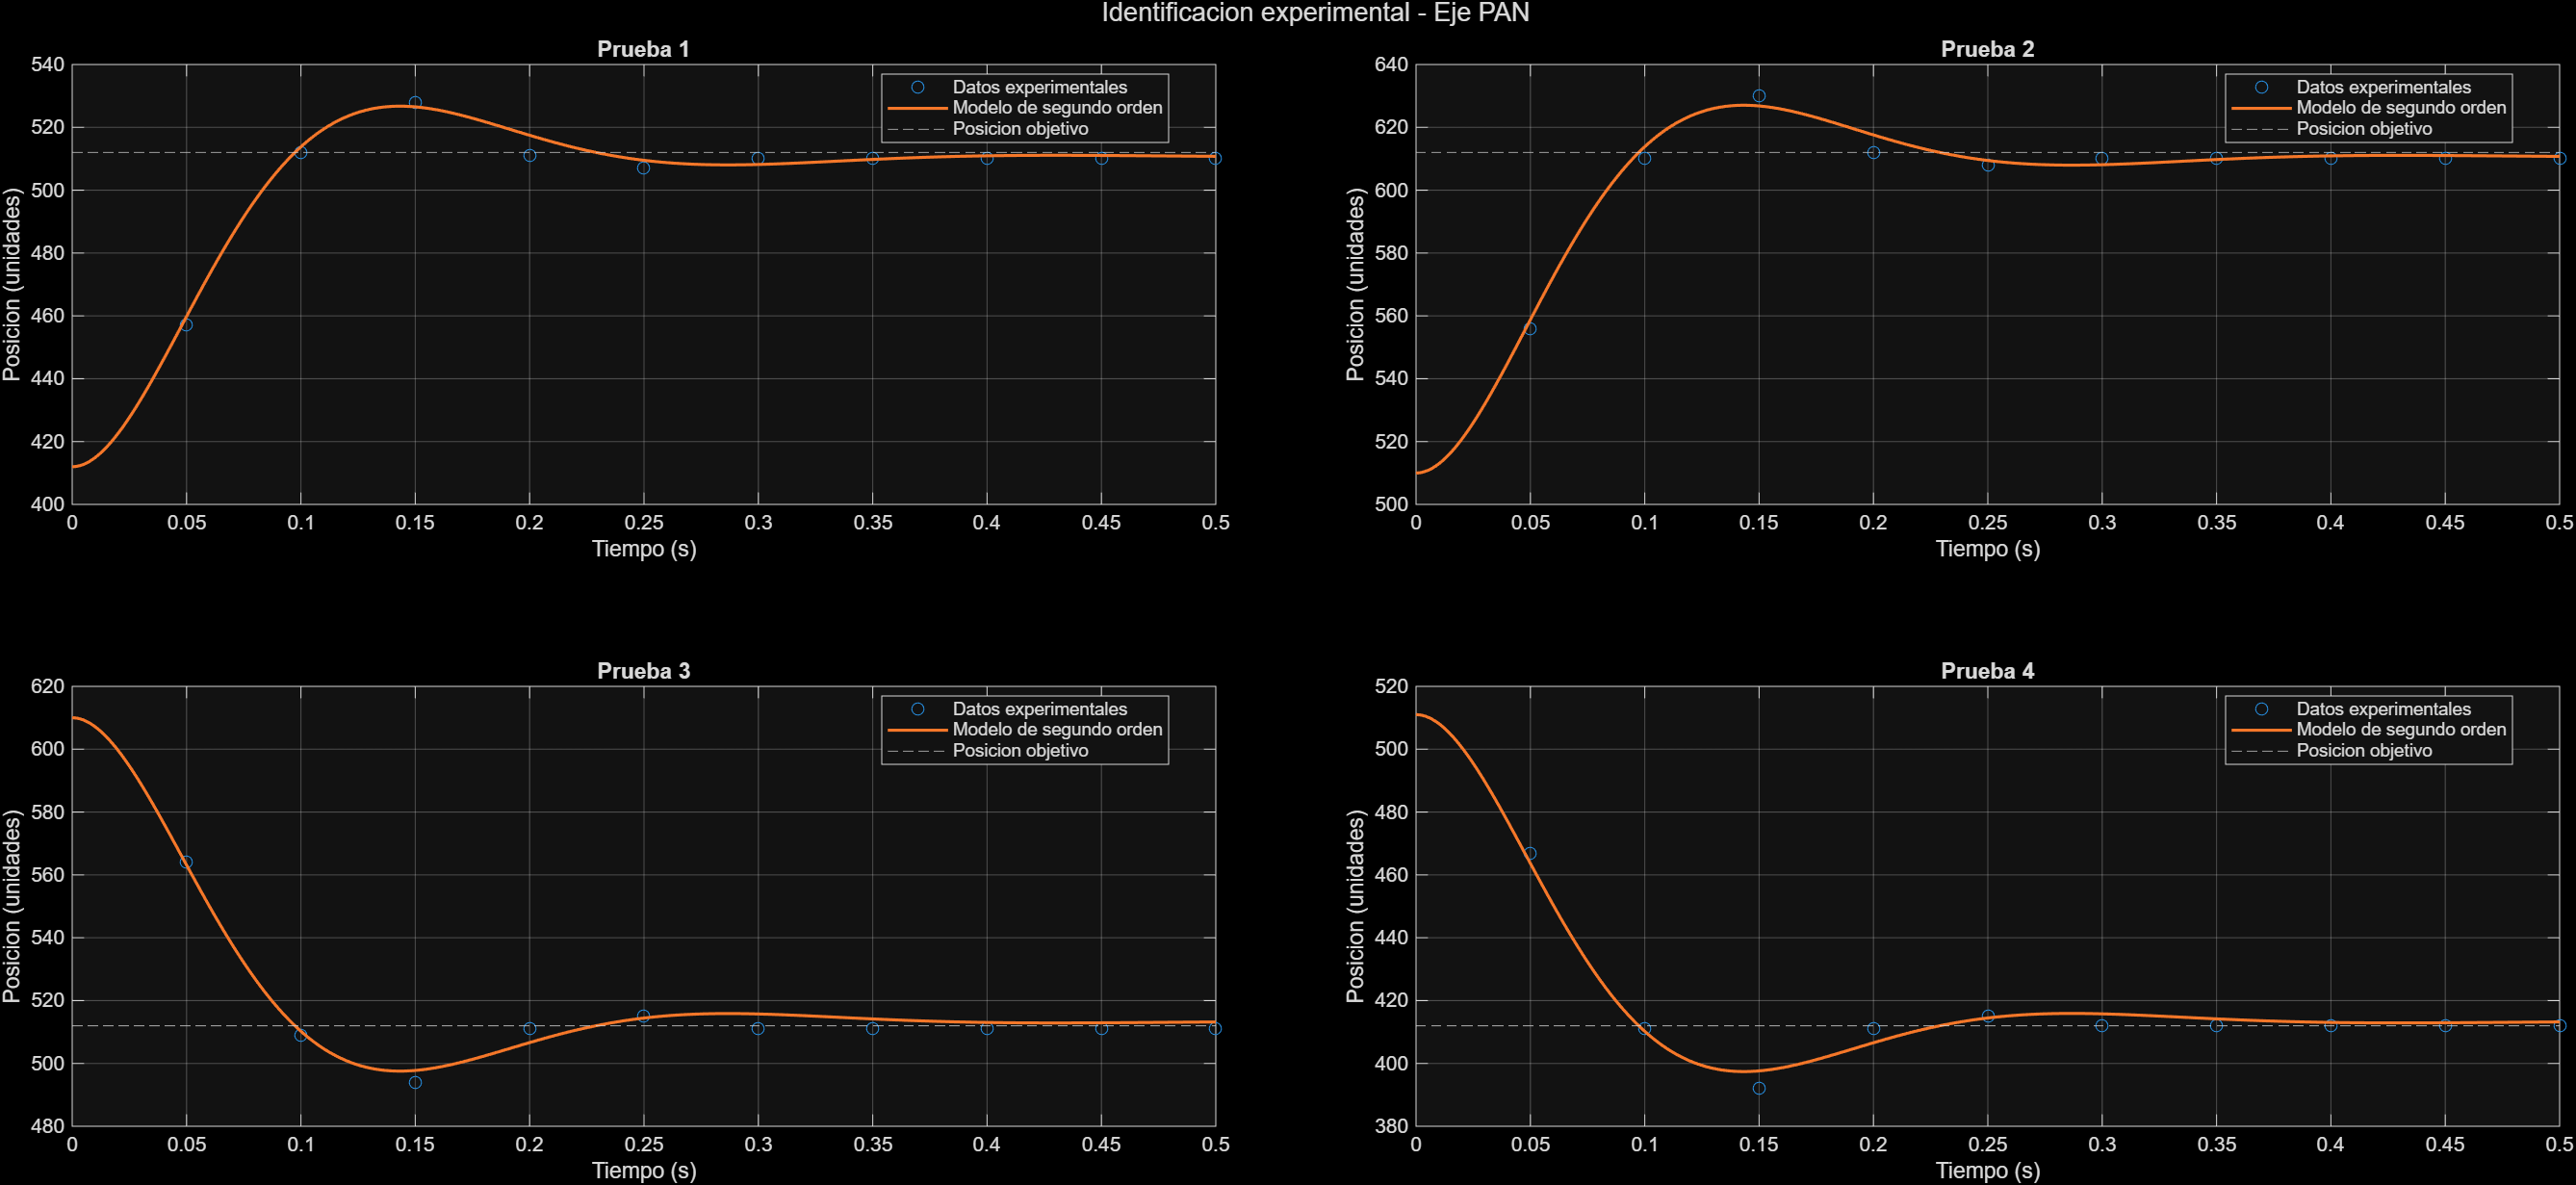
\includegraphics[width=0.9\linewidth]{Figuras/Identificacion PAN.png}
    \caption{Respuesta experimental y ajuste de identificación para el eje horizontal (\emph{Pan}).}
    \label{fig:ident_pan}
\end{figure}

\begin{figure}[H]
    \centering
    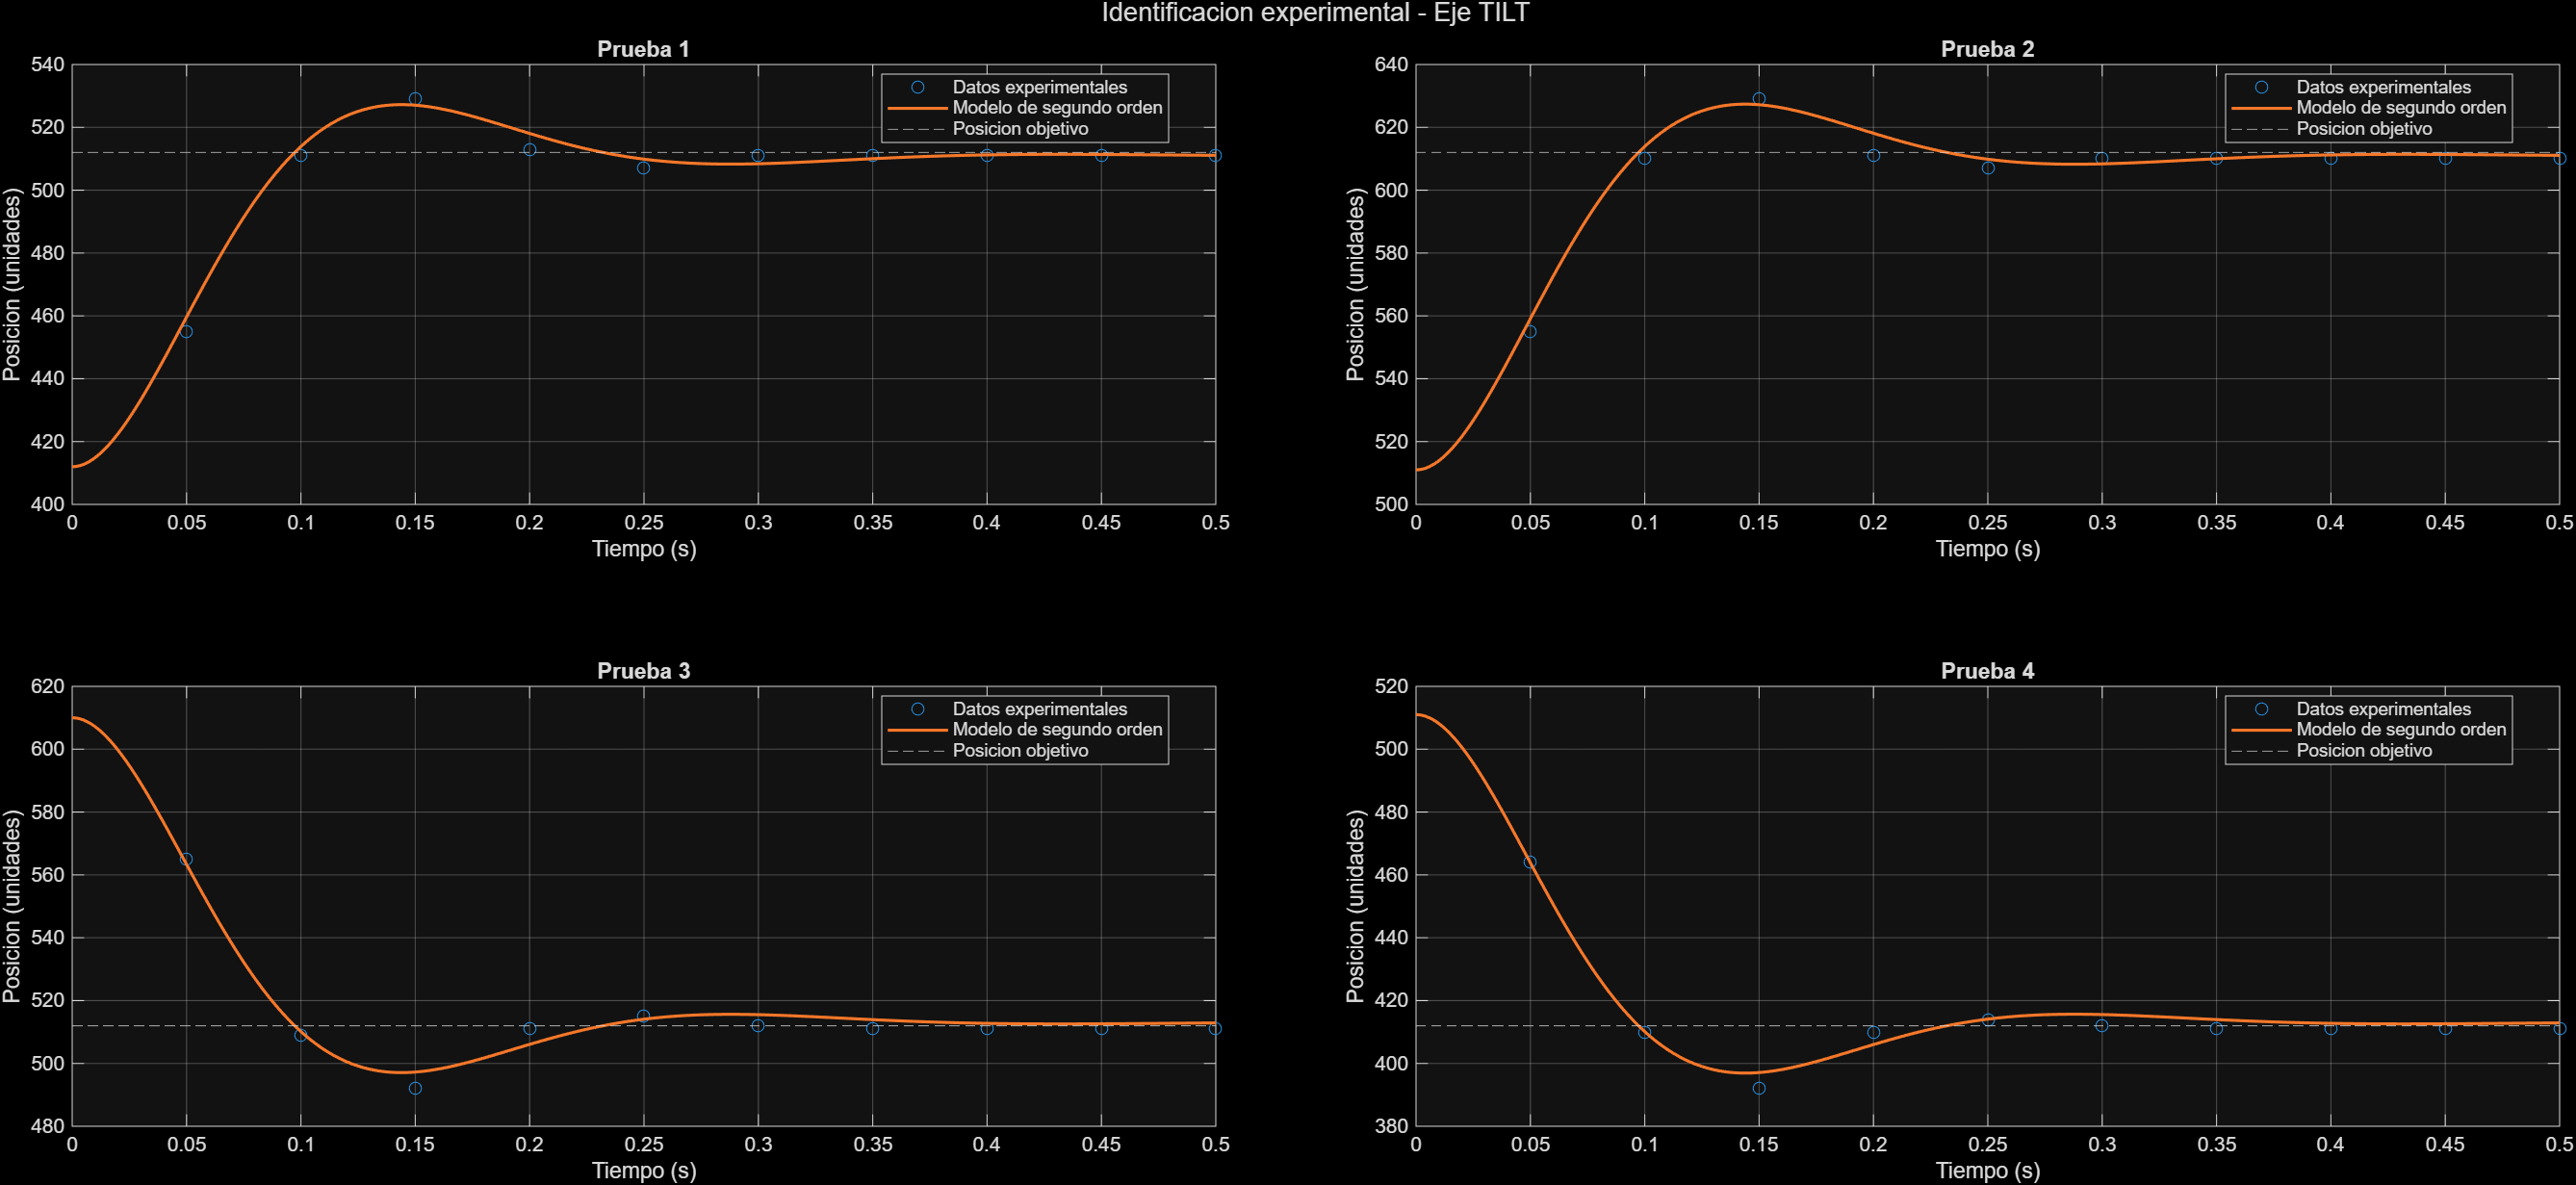
\includegraphics[width=0.9\linewidth]{Figuras/Identificacion TILT.png}
    \caption{Respuesta experimental y ajuste de identificación para el eje vertical (\emph{Tilt}).}
    \label{fig:ident_tilt}
\end{figure}

De manera paralela, para caracterizar el subsistema de sensado con las cuatro fotoresistencias, se empleó igualmente código en C++ en Arduino IDE sobre la placa ArbotiX-M, muestreando las lecturas ADC de cada sensor cada $250\text{ ms}$ y guardando las mediciones en archivos CSV para su procesamiento en MATLAB. Las pruebas incluyeron condiciones de oscuridad, iluminación ambiental (sin la fuente luminosa objetivo) y desplazamientos angulares con variaciones de $10^\circ$ en cada dirección (izquierda, derecha, arriba y abajo), evaluando posiciones en el rango de $-30^\circ$ a $+30^\circ$ (por ejemplo, izquierda $10^\circ$, $20^\circ$ y $30^\circ$), con promedios calculados sobre las últimas $N=10$ muestras de cada condición.

En el registro de las fotoresistencias, cada fila incluye el identificador de iteración (\texttt{Iteracion}), el índice de muestra consecutivo (\texttt{N}) tomado cada $250\text{ ms}$ y las lecturas ADC de los cuatro sensores (\texttt{S1}, \texttt{S2}, \texttt{S3} y \texttt{S4}). En el Cuadro~\ref{tab:muestra_ldr_centrada} se muestra un ejemplo de la serie de $20$ muestras obtenida con la fuente LED centrada, donde se aprecia la estabilización progresiva de las lecturas tras el inicio de la captura.

\begin{table}[H]
    \centering
    \caption{Registro de ejemplo de mediciones ADC de las fotoresistencias con la fuente LED centrada (Iteración 1, muestreo cada $250\text{ ms}$).}
    \label{tab:muestra_ldr_centrada}
    \begin{tabular}{cccccc}
        \toprule
        \textbf{Iteración} & \textbf{N} & \textbf{S1} & \textbf{S2} & \textbf{S3} & \textbf{S4} \\
        \midrule
        1 & 1  & 903.0 & 928.7 & 715.1 & 575.5 \\
        1 & 2  & 902.0 & 928.0 & 800.6 & 699.6 \\
        1 & 3  & 901.0 & 927.0 & 820.4 & 748.0 \\
        1 & 4  & 900.0 & 927.0 & 825.8 & 764.6 \\
        1 & 5  & 899.0 & 926.0 & 826.4 & 769.7 \\
        1 & 6  & 899.0 & 925.5 & 827.0 & 772.4 \\
        1 & 7  & 896.1 & 923.8 & 826.1 & 772.0 \\
        1 & 8  & 896.0 & 923.2 & 826.0 & 772.1 \\
        1 & 9  & 899.0 & 924.0 & 827.0 & 773.4 \\
        1 & 10 & 901.9 & 925.0 & 827.5 & 774.1 \\
        1 & 11 & 902.0 & 923.0 & 826.9 & 773.8 \\
        1 & 12 & 901.0 & 923.0 & 826.9 & 773.6 \\
        1 & 13 & 902.0 & 923.4 & 827.2 & 774.2 \\
        1 & 14 & 900.9 & 922.0 & 826.3 & 774.0 \\
        1 & 15 & 899.0 & 920.0 & 825.4 & 773.6 \\
        1 & 16 & 900.7 & 918.9 & 823.8 & 771.8 \\
        1 & 17 & 902.3 & 921.0 & 825.7 & 772.9 \\
        1 & 18 & 903.0 & 923.0 & 827.3 & 774.7 \\
        1 & 19 & 902.1 & 923.6 & 827.9 & 775.7 \\
        1 & 20 & 901.0 & 923.8 & 828.5 & 775.6 \\
        \bottomrule
    \end{tabular}
\end{table}

Asimismo, las curvas experimentales de calibración angular obtenidas en MATLAB para el error horizontal normalizado ($e_x$) frente al ángulo \emph{Pan} (en grados) y para el error vertical normalizado ($e_y$) frente al ángulo \emph{Tilt} (en grados) se presentan en las Figuras~\ref{fig:cal_pan} y~\ref{fig:cal_tilt}, respectivamente.

\begin{figure}[H]
    \centering
    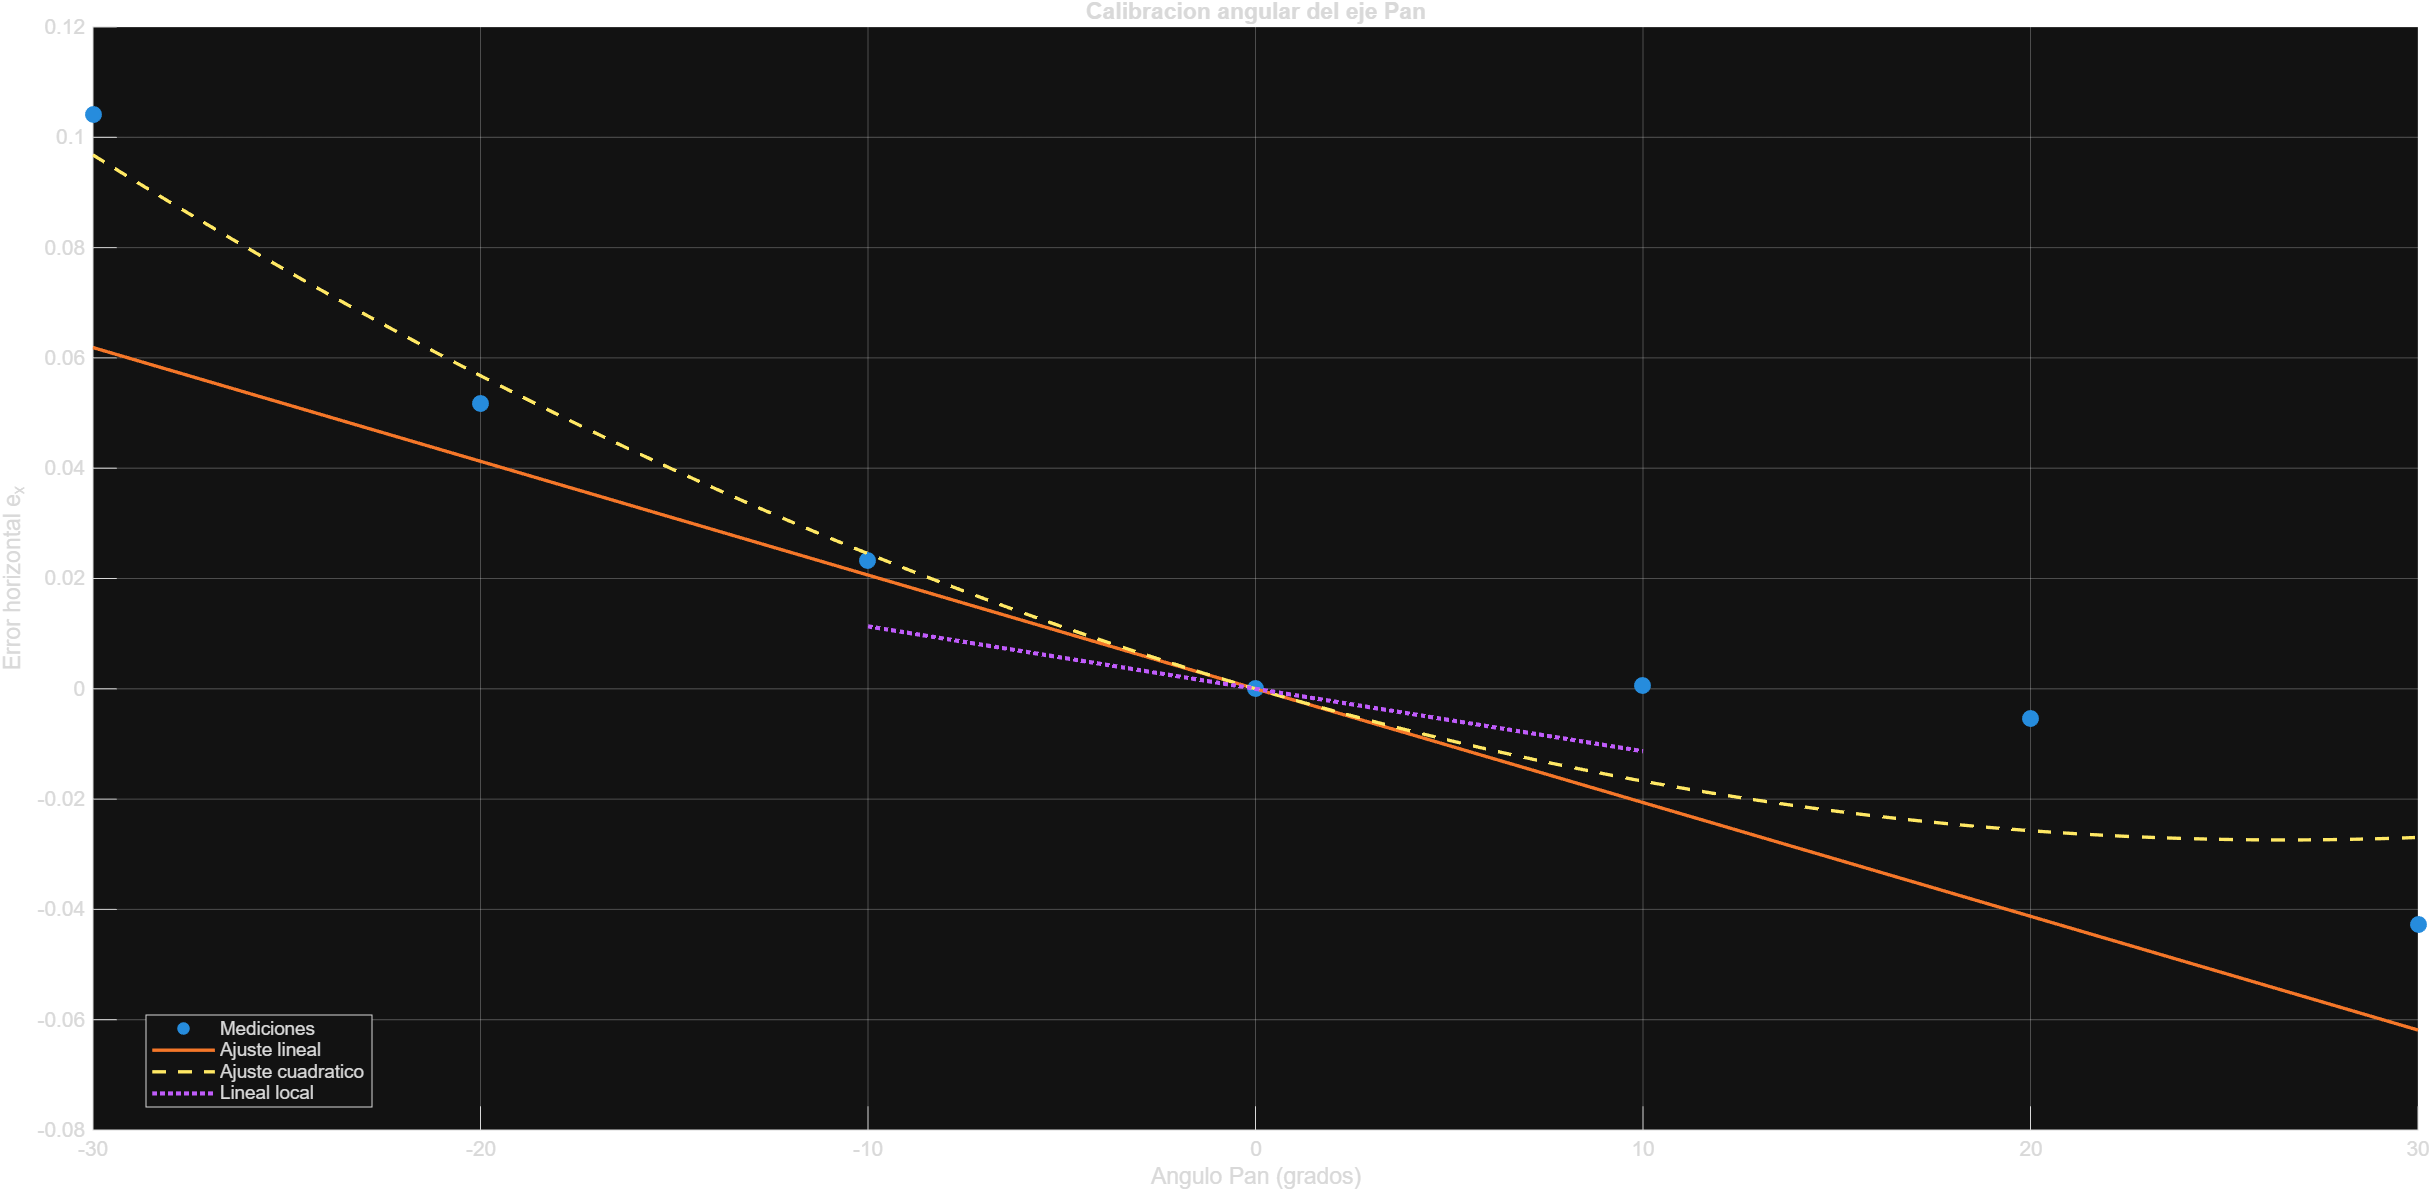
\includegraphics[width=0.9\linewidth]{Figuras/Calibracion angular Pan.png}
    \caption{Calibración angular del error horizontal normalizado ($e_x$) respecto al ángulo \emph{Pan} (en grados).}
    \label{fig:cal_pan}
\end{figure}

\begin{figure}[H]
    \centering
    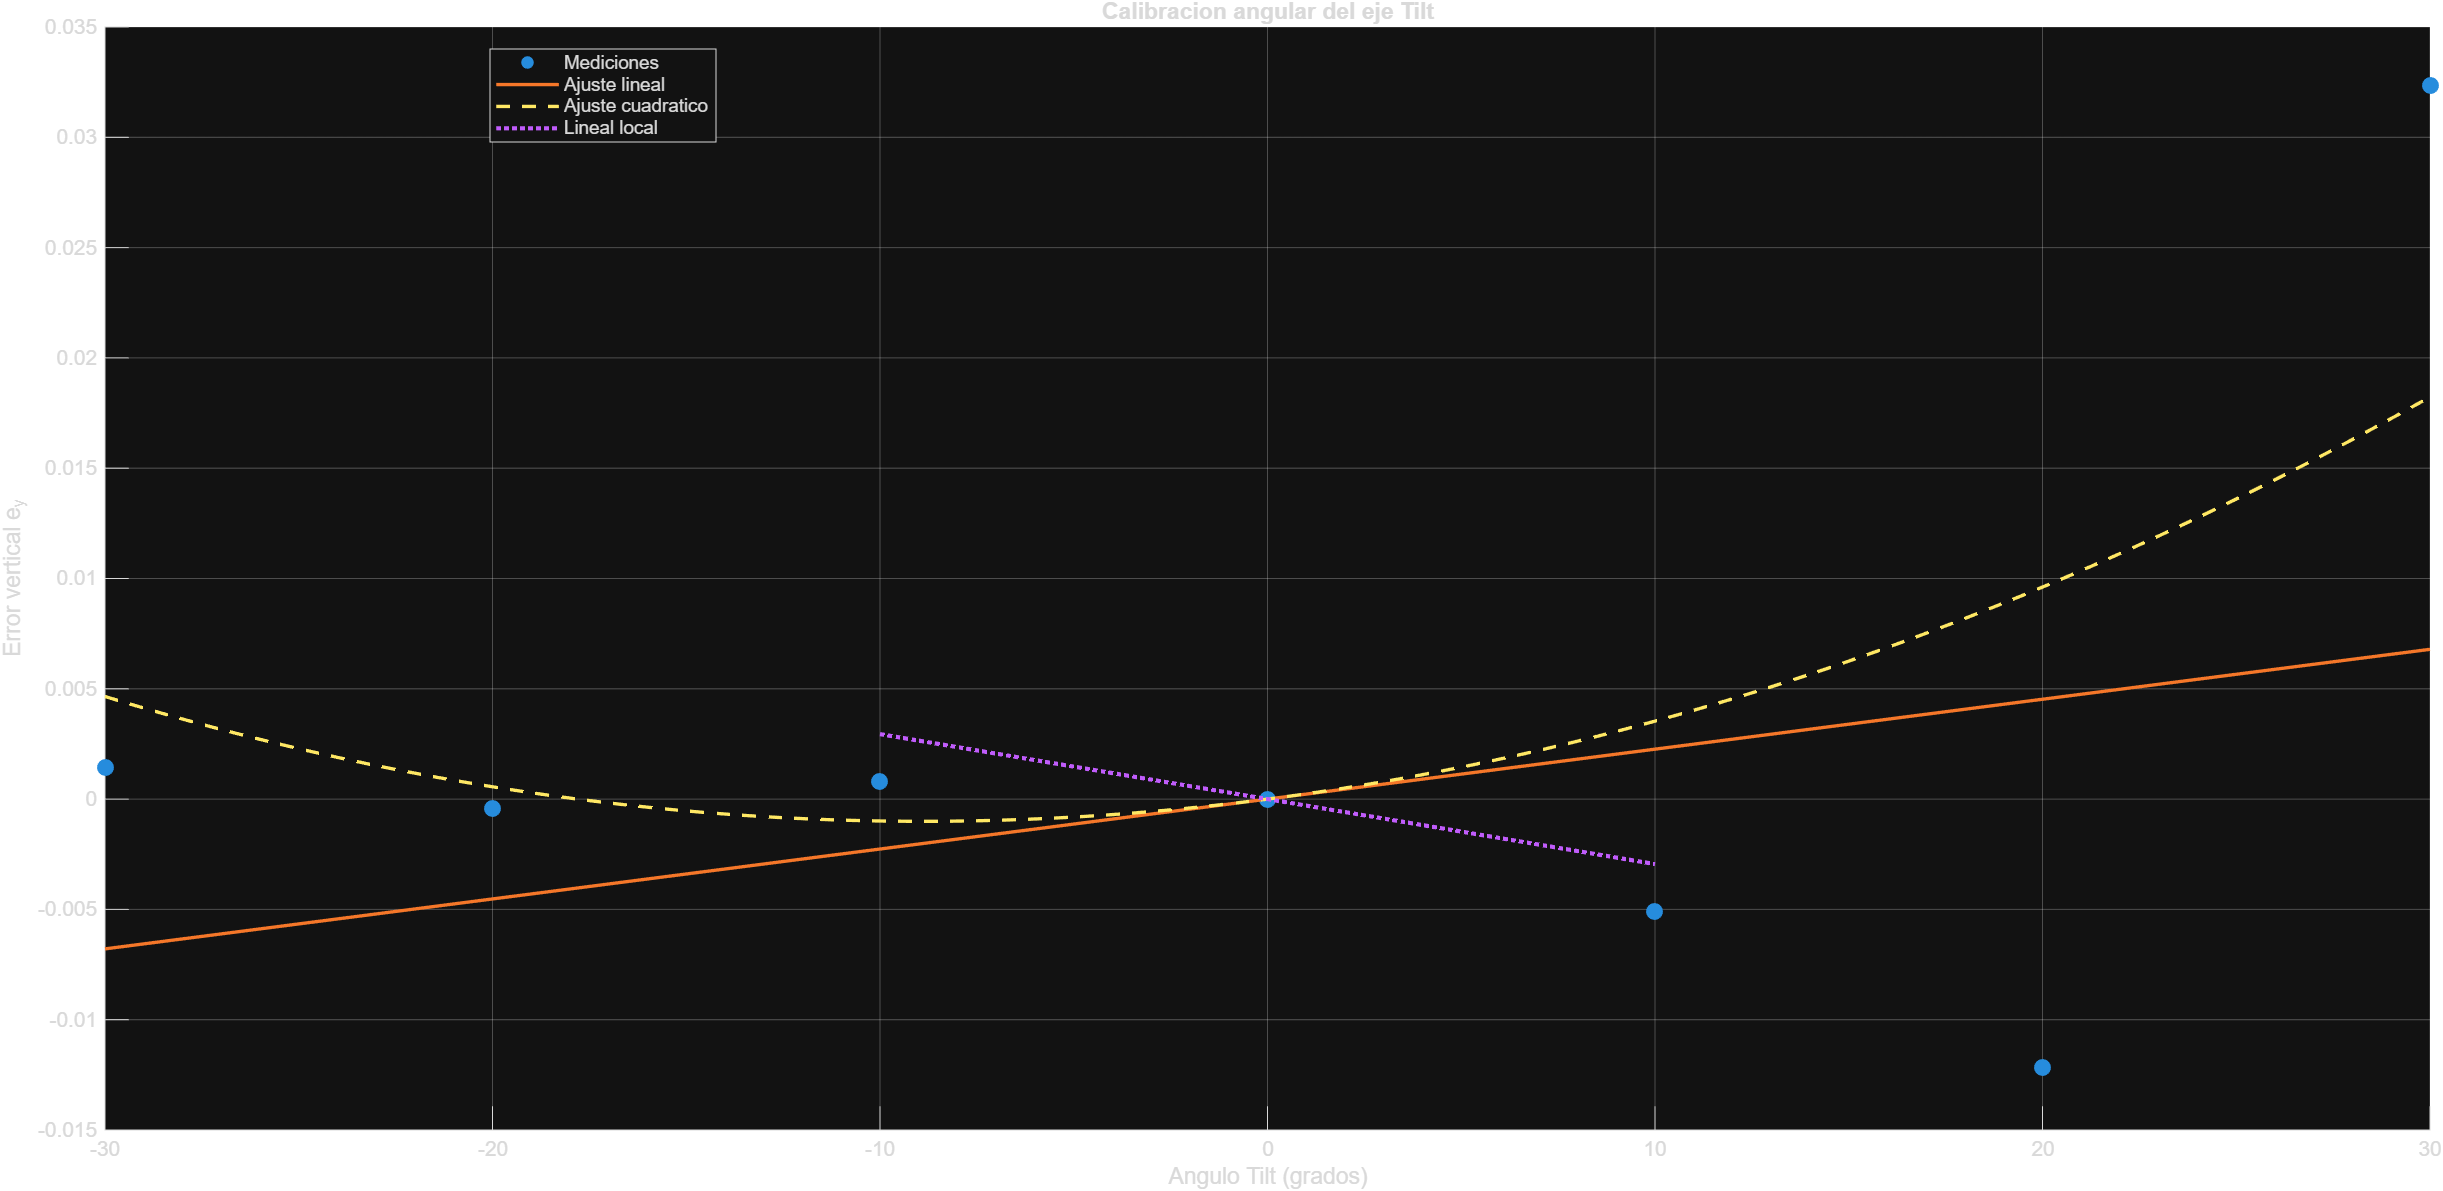
\includegraphics[width=0.9\linewidth]{Figuras/Calibracion angular Tilt.png}
    \caption{Calibración angular del error vertical normalizado ($e_y$) respecto al ángulo \emph{Tilt} (en grados).}
    \label{fig:cal_tilt}
\end{figure}

\subsection{Modelo Real}
A partir del procesamiento y ajuste de las curvas experimentales en MATLAB, se identificaron los parámetros característicos de segundo orden para ambos ejes de movimiento. En el Cuadro~\ref{tab:parametros_identificados} se resumen las constantes dinámicas obtenidas, evidenciando un comportamiento subamortiguado ($\zeta \approx 0.50$) muy consistente entre los dos servomotores.

\begin{table}[H]
    \centering
    \caption{Parámetros dinámicos experimentales identificados en MATLAB para los ejes \emph{Pan} y \emph{Tilt}.}
    \label{tab:parametros_identificados}
    \begin{tabular}{lcc}
        \toprule
        \textbf{Parámetro} & \textbf{Eje Horizontal (\emph{Pan})} & \textbf{Eje Vertical (\emph{Tilt})} \\
        \midrule
        Ganancia estática ($K$) & $0.98669$ & $0.98970$ \\
        Coeficiente de amortiguamiento ($\zeta$) & $0.50026$ & $0.49847$ \\
        Frecuencia natural ($\omega_n$) & $25.31960\text{ rad/s}$ & $25.17597\text{ rad/s}$ \\
        Frecuencia amortiguada ($\omega_d$) & $21.92364\text{ rad/s}$ & $21.82524\text{ rad/s}$ \\
        Tiempo de establecimiento ($t_s$) & $0.31580\text{ s}$ & $0.31874\text{ s}$ \\
        Polos dominantes ($s_{1,2}$) & $-12.6663 \pm j21.9236$ & $-12.5494 \pm j21.8252$ \\
        \bottomrule
    \end{tabular}
\end{table}

Sustituyendo los valores identificados en la estructura teórica de segundo orden, las funciones de transferencia experimentales de la planta en tiempo continuo quedan definidas como:

\begin{align}
G_{\text{PAN}}(s) &= \frac{\Theta_x(s)}{U_x(s)} = \frac{632.5}{s^2 + 25.33s + 641.1} \\
G_{\text{TILT}}(s) &= \frac{\Theta_y(s)}{U_y(s)} = \frac{627.3}{s^2 + 25.10s + 633.8}
\end{align}

De manera equivalente, la representación en espacio de estados real para cada eje se obtiene sustituyendo los coeficientes numéricos en las matrices del sistema:

\begin{equation}
\dot{\mathbf{x}}_{\text{PAN}} = \begin{bmatrix} 0 & 1 \\ -641.1 & -25.33 \end{bmatrix} \mathbf{x}_{\text{PAN}} + \begin{bmatrix} 0 \\ 632.5 \end{bmatrix} u_x, \quad y_x = \begin{bmatrix} 1 & 0 \end{bmatrix} \mathbf{x}_{\text{PAN}}
\end{equation}

\begin{equation}
\dot{\mathbf{x}}_{\text{TILT}} = \begin{bmatrix} 0 & 1 \\ -633.8 & -25.10 \end{bmatrix} \mathbf{x}_{\text{TILT}} + \begin{bmatrix} 0 \\ 627.3 \end{bmatrix} u_y, \quad y_y = \begin{bmatrix} 1 & 0 \end{bmatrix} \mathbf{x}_{\text{TILT}}
\end{equation}

A partir de la similitud dinámica observada entre ambos ejes, también es posible definir un modelo promedio general de segundo orden tomando las medias aritméticas de los parámetros identificados para \emph{Pan} y \emph{Tilt}:

\begin{align}
K_{\text{prom}} &= 0.988195 \\
\zeta_{\text{prom}} &= 0.499365 \\
\omega_{n,\text{prom}} &= 25.247785\text{ rad/s}
\end{align}

De este modo, se obtiene la función de transferencia generalizada para los servomotores:

\begin{equation}
\boxed{
G(s) = \frac{629.7}{s^2 + 25.22s + 637.4}
}
\end{equation}

Este modelo unificado resulta práctico para realizar análisis preliminares y diseños de control base antes de ajustar o refinar cada eje por separado.

Por otra parte, en el subsistema de fotoresistencias, el procesamiento en MATLAB sobre los datos registrados permitió obtener los parámetros de compensación en oscuridad ($O_1 = 4.18$, $O_2 = 33.03$, $O_3 = 94.38$ y $O_4 = 127.30$ unidades ADC), las lecturas ambientales ($A_1 = 818.41$, $A_2 = 861.18$, $A_3 = 776.87$ y $A_4 = 730.71$ ADC; corregidas: $A_{1,c} = 814.23$, $A_{2,c} = 828.15$, $A_{3,c} = 682.49$ y $A_{4,c} = 603.41$ ADC) y las ganancias individuales de calibración respecto al promedio central $\overline{S}_{c,0} = 815.36$ ADC:

\begin{align}
U_1(t) &= 0.879711\left[S_1(t) - 4.18\right], &
U_2(t) &= 0.891191\left[S_2(t) - 33.03\right] \\
U_3(t) &= 1.081451\left[S_3(t) - 94.38\right], &
U_4(t) &= 1.224761\left[S_4(t) - 127.30\right]
\end{align}

A partir de los ajustes por mínimos cuadrados forzados al origen en el rango completo de $\pm 30^\circ$ (con ángulos en grados), se obtuvieron para el eje \emph{Pan} los modelos lineal y cuadrático:

\begin{equation}
e_x(\Delta\theta_x) = -0.00206250\Delta\theta_x \qquad (R^2 = 0.70298,\; \text{RMSE} = 0.023878)
\end{equation}

\begin{equation}
e_x(\Delta\theta_x) = 0.00003881\Delta\theta_x^2 - 0.00206250\Delta\theta_x \qquad (R^2 = 0.92264,\; \text{RMSE} = 0.012186)
\end{equation}

Mientras que para el eje \emph{Tilt} en el rango de $\pm 30^\circ$ se obtuvieron:

\begin{equation}
e_y(\Delta\theta_y) = 0.00022632\Delta\theta_y \qquad (R^2 = 0.08705,\; \text{RMSE} = 0.012417)
\end{equation}

\begin{equation}
e_y(\Delta\theta_y) = 0.00001271\Delta\theta_y^2 + 0.00022632\Delta\theta_y \qquad (R^2 = 0.35499,\; \text{RMSE} = 0.010437)
\end{equation}

En el entorno local de pequeña señal de $\pm 10^\circ$, las expresiones lineales identificadas para cada eje (con ángulos en grados) corresponden a:

\begin{equation}
e_x(\Delta\theta_x) = -0.00113199\Delta\theta_x \qquad (R^2 = 0.19336,\; \text{RMSE} = 0.009708)
\end{equation}

\begin{equation}
e_y(\Delta\theta_y) = -0.00029447\Delta\theta_y \qquad (R^2 = 0.54377,\; \text{RMSE} = 0.001764)
\end{equation}

En el Cuadro~\ref{tab:parametros_ldr} se resumen los parámetros identificados del subsistema de sensado y su acoplamiento experimental.

\begin{table}[H]
    \centering
    \caption{Resumen de parámetros experimentales identificados para el subsistema de fotoresistencias.}
    \label{tab:parametros_ldr}
    \begin{tabular}{lcc}
        \toprule
        \textbf{Parámetro} & \textbf{Valor} & \textbf{Unidad} \\
        \midrule
        $O_1, O_2, O_3, O_4$ & $4.18,\; 33.03,\; 94.38,\; 127.30$ & $\text{ADC}$ \\
        $G_1, G_2, G_3, G_4$ & $0.879711,\; 0.891191,\; 1.081451,\; 1.224761$ & Adim. \\
        $K_{xx}$ (ganancia estática \emph{Pan}) & $-0.06485802$ & $\text{rad}^{-1}$ \\
        $K_{yy}$ (ganancia estática \emph{Tilt}) & $-0.01687204$ & $\text{rad}^{-1}$ \\
        $K_{xy}$ / $K_{yx}$ & $-0.0223$ / $-0.0627$ & $\text{rad}^{-1}$ \\
        Acoplamiento \emph{Pan} $\rightarrow$ \emph{Tilt} ($C_{x\rightarrow y}$) & $96.656$ & $\%$ \\
        Acoplamiento \emph{Tilt} $\rightarrow$ \emph{Pan} ($C_{y\rightarrow x}$) & $131.898$ & $\%$ \\
        \bottomrule
    \end{tabular}
\end{table}

Expresando las ganancias estáticas en radianes mediante la conversión $K_{s,\mathrm{rad}} = K_{s,\mathrm{deg}}(180/\pi)$, se tienen las ganancias locales $K_{xx} \approx -0.06485802\text{ rad}^{-1}$ y $K_{yy} \approx -0.01687204\text{ rad}^{-1}$. Las funciones de transferencia estáticas equivalentes consideradas en el modelado son:

\begin{align}
\boxed{H_x(s) = \frac{E_x(s)}{\Delta\Theta_x(s)} \approx -0.06485802} \\
\boxed{H_y(s) = \frac{E_y(s)}{\Delta\Theta_y(s)} \approx -0.01687204}
\end{align}

Sin embargo, debido a la asimetría y a los elevados acoplamientos cruzados ($C_{x\rightarrow y} = 96.656\%$ y $C_{y\rightarrow x} = 131.898\%$), el modelo local acoplado en radianes queda dado por:
\begin{equation}
\begin{bmatrix} e_x(t) \\ e_y(t) \end{bmatrix} \approx
\begin{bmatrix} -0.0649 & -0.0223 \\ -0.0627 & -0.0169 \end{bmatrix}
\begin{bmatrix} \Delta\theta_x(t) \\ \Delta\theta_y(t) \end{bmatrix}
\end{equation}

A partir de los resultados obtenidos durante la caracterización experimental del subsistema de sensado, se determinó que el comportamiento de los sensores presenta características no lineales y asimétricas dentro del rango angular evaluado. Si bien el modelo cuadrático proporcionó un mejor ajuste respecto al modelo lineal en el eje \emph{Pan}, ninguno de los modelos globales logró representar satisfactoriamente el comportamiento de ambos ejes.

Considerando que el objetivo principal del sistema consiste en localizar la fuente luminosa y mantener su orientación hacia esta, se seleccionó un modelo lineal de pequeña señal alrededor del punto de operación correspondiente a una desviación angular de $0^\circ$. En las proximidades de dicho punto, se busca que las desviaciones angulares sean reducidas, por lo que resulta conveniente emplear una aproximación lineal de la respuesta de los sensores.

Para la identificación de este modelo se utilizaron las mediciones correspondientes al intervalo angular comprendido entre $-10^\circ$ y $+10^\circ$, mediante un ajuste por mínimos cuadrados restringido a pasar por el origen. Esta aproximación permite representar el subsistema de sensado mediante ganancias estáticas equivalentes, facilitando su integración con las funciones de transferencia de los actuadores y la aplicación de técnicas clásicas de diseño de sistemas de control.

\section{Diseño e Implementación del Controlador}



\section{Simulaciones}

\section{Resultados y Análisis}

\section{Conclusiones}

\printbibliography[title={Bibliografía},heading=bibintoc]

\end{document}
